\iffalse
\documentclass[12pt,twocolumn]{article}
\usepackage[margin=0.5in]{geometry}
\def\inputGnumerictable{}
\usepackage[cmex10]{amsmath}
\usepackage{gensymb}
\usepackage{graphicx}
\usepackage{amsthm}
\usepackage{mathrsfs}
\usepackage{txfonts}
\usepackage{cite}
\usepackage{cases}
\usepackage{subfig}
\usepackage[breaklinks=true]{hyperref}
\usepackage{listings}
\usepackage[latin1]{inputenc}
    \usepackage{color}                                         
    \usepackage{array}                                         
    \usepackage{longtable}                       
    \usepackage{calc}                                            
    \usepackage{multirow}                                       
    \usepackage{hhline}                                           
    \usepackage{ifthen}                                           
    \usepackage{amssymb}
\providecommand{\pr}[1]{\ensuremath{\pr\left(#1\right)}}
\newcommand*{\Comb}[2]{{}^{#1}C_{#2}}%
\title{
Probability Assignment
}
\author{GINNA SHREYANI}
\date{}
\providecommand{\pr}[1]{\ensuremath{\pr\left(#1\right)}}

\begin{document}
\maketitle

\textbf{11.16.3.2}\\
\subsection*{Solution}
\fi
By using binomial distribution, the desired probability is given by 
\iffalse

we can find the probability of atleast one tail occurs hen a coin is tossed twice.\\
Here we are assuming when ever a tail shows up it is a success(1)\\
The Binomial Distribution: Let
\begin{align}
	Y &= \sum_{i=1}^n X_i
         \label{eq-1}
\end{align}
where n is the total number of times the coin is tossed. Then X has a binomial distribution. Then, for
\begin{align}
	&p_{X_i}(n){\stackrel{z}{\rightleftharpoons}}P_{X_i}(z),
     \label{eq-2}
\end{align}
yielding
\begin{align}
	P_{X_i}(Z) &= 1-p+pz^{-1}
	\label{eq-3}
\end{align}
Since $X_i$ are i.i.d.,
\begin{align}
	P_X(Z)&=(1-p+pz^{-1})^n\\
	&=\sum_{k=0}^n{\Comb{n}{k}p^{k}(1-p)^{n-k}}
\end{align}
\[
	p_X(k)=
	\begin{cases}
		\Comb{n}{k}p^{n-k}(1-p)^k,& \text{if } 0\leq k\leq n\\
		0,& \text{otherwise}
	\end{cases}
\]
As a result it is written as
\begin{align}
	\label{eq-6}
	p_X(k) &=\binom nk p^{k}(1-p)^{n-k}
\end{align}
The cumulative distribution function of X is defined as
\begin{align}
	F_X(r) &=\pr(X\leq r) = \sum_{k=0}^r\binom nk p^{k}(1-p)^{n-k}
	\label{eq-7}
\end{align}
Therefore, we get the number of trails i.e., the number of times the coin is tossed and the probability of getting atleast one tail is sum of the probability of getting one tail and probability of getting two tails.
The probability of getting a tail when a coin is tossed is 0.5.
\begin{align}
	n &= 2\\
	r &= 1,2\\
	p &= 0.5
\end{align}
Therefore,
\fi
\begin{align}
	\pr{Y\geq 1}=\sum_{k=1}^2 \binom nk p^k(1-p)^{n-k}
	= \frac{3}{4}
\end{align}
upon substituting $p = \frac{1}{2}$.
\iffalse
Therefore,the probability of getting atleast one tail whenthe coinis tossed twice is 0.75.\\
\begin{table}[h]
	%%%%%%%%%%%%%%%%%%%%%%%%%%%%%%%%%%%%%%%%%%%%%%%%%%%%%%%%%%%%%%%%%%%%%%
%%                                                                  %%
%%  This is a LaTeX2e table fragment exported from Gnumeric.        %%
%%                                                                  %%
%%%%%%%%%%%%%%%%%%%%%%%%%%%%%%%%%%%%%%%%%%%%%%%%%%%%%%%%%%%%%%%%%%%%%%
\begin{align}
    \begin{tabular}{|l|l|}\hline
        Red ball from Bag I:	    &\pr{X=1,Y=1}=$\frac{3}{7}$\\\hline
        Black ball from Bag I:	&\pr{X=1,Y=2}=$\frac{4}{7}$\\\hline
        Red ball from Bag II:	&\pr{X=2,Y=1}=$\frac{31}{70}$\\\hline
        Black ball from Bag II: &\pr{X=2,Y=2}=$\frac{39}{70}$\\\hline
        \end{tabular}
    \end{align}
\end{table}

\begin{figure}[h]
    \centering
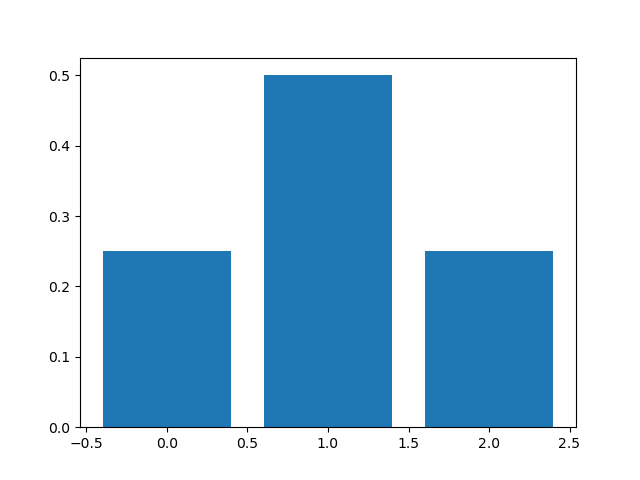
\includegraphics[width=\columnwidth]{fig/11.16.3.2.png}
\end{figure}
This is the code: \href{https://github.com/ShreyaniReddy/IITH-FWC/blob/main/probability/11.16.3.2/codes/11.16.3.2.py}{Code}
\end{document}
\fi
